% Content for DCT Results subsection
% This file is included in the main conference paper via % Content for DCT Results subsection
% This file is included in the main conference paper via % Content for DCT Results subsection
% This file is included in the main conference paper via % Content for DCT Results subsection
% This file is included in the main conference paper via \input{DCTResults}

We claimed in \ref{methodsec:fourier} that DCT is superior to DFT for image compression. To see this clearly, Fig. \ref{fig:dctvsdft} shows how DCT achieves much higher compression ratios at equivalent PSNR values across all datasets. For example, at a PSNR of 30 dB, the DFT achieves CR$\approx5$ across all datasets, while DCT has CR$\approx10$, even closer to 15 for Aerial Images. 

\begin{figure}
    \centering
    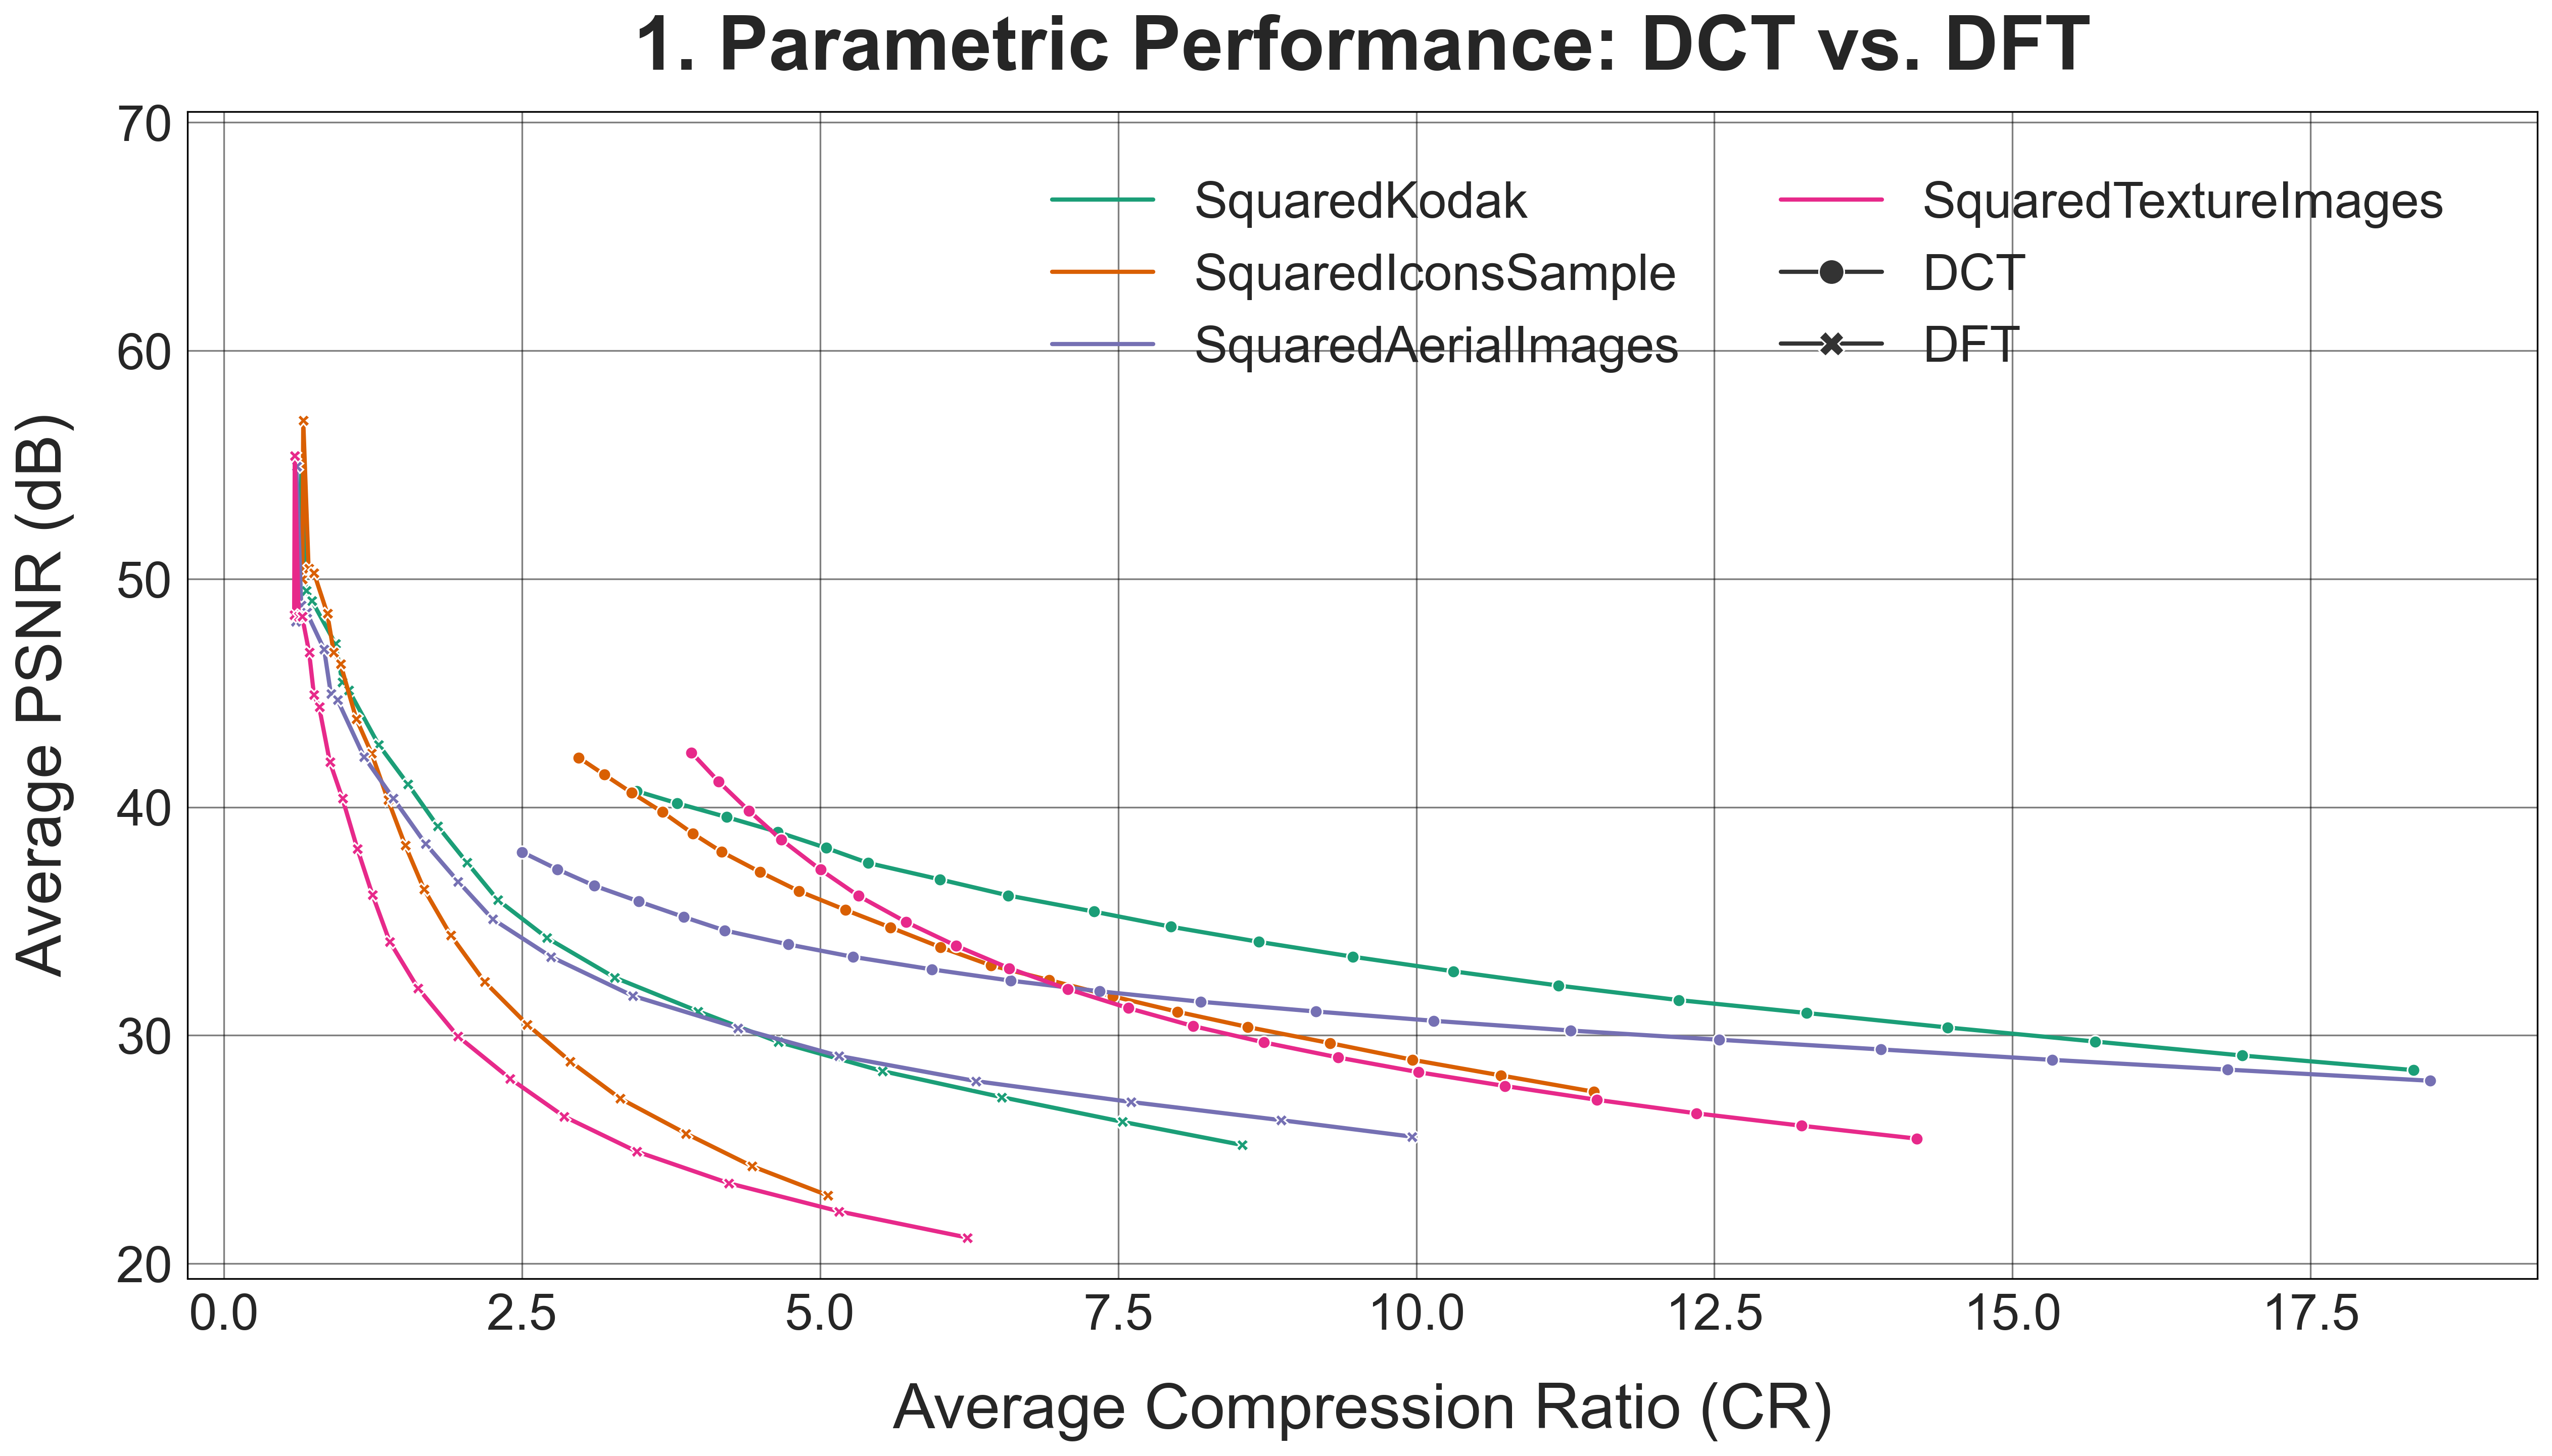
\includegraphics[width=1\linewidth]{results/plots/plot_5_parametric_DCT_vs_DFT.png}
    \caption{Different levels of quantization on sample image with compression ratio.}
    \label{fig:dctvsdft}
\end{figure}

Notably, in \ref{resultssec:col} it appears that the DCT outperforms all transform algorithms, not just the DFT. This comparison is slightly unfair since an additional step RLE was added to the entropy coding for DCT as described in \ref{methodsec:entropy}. Fig. \ref{fig:dctcrvsdcr} shows how the compression ratios change without RLE present for a more fair comparison.

\begin{figure}
    \centering
    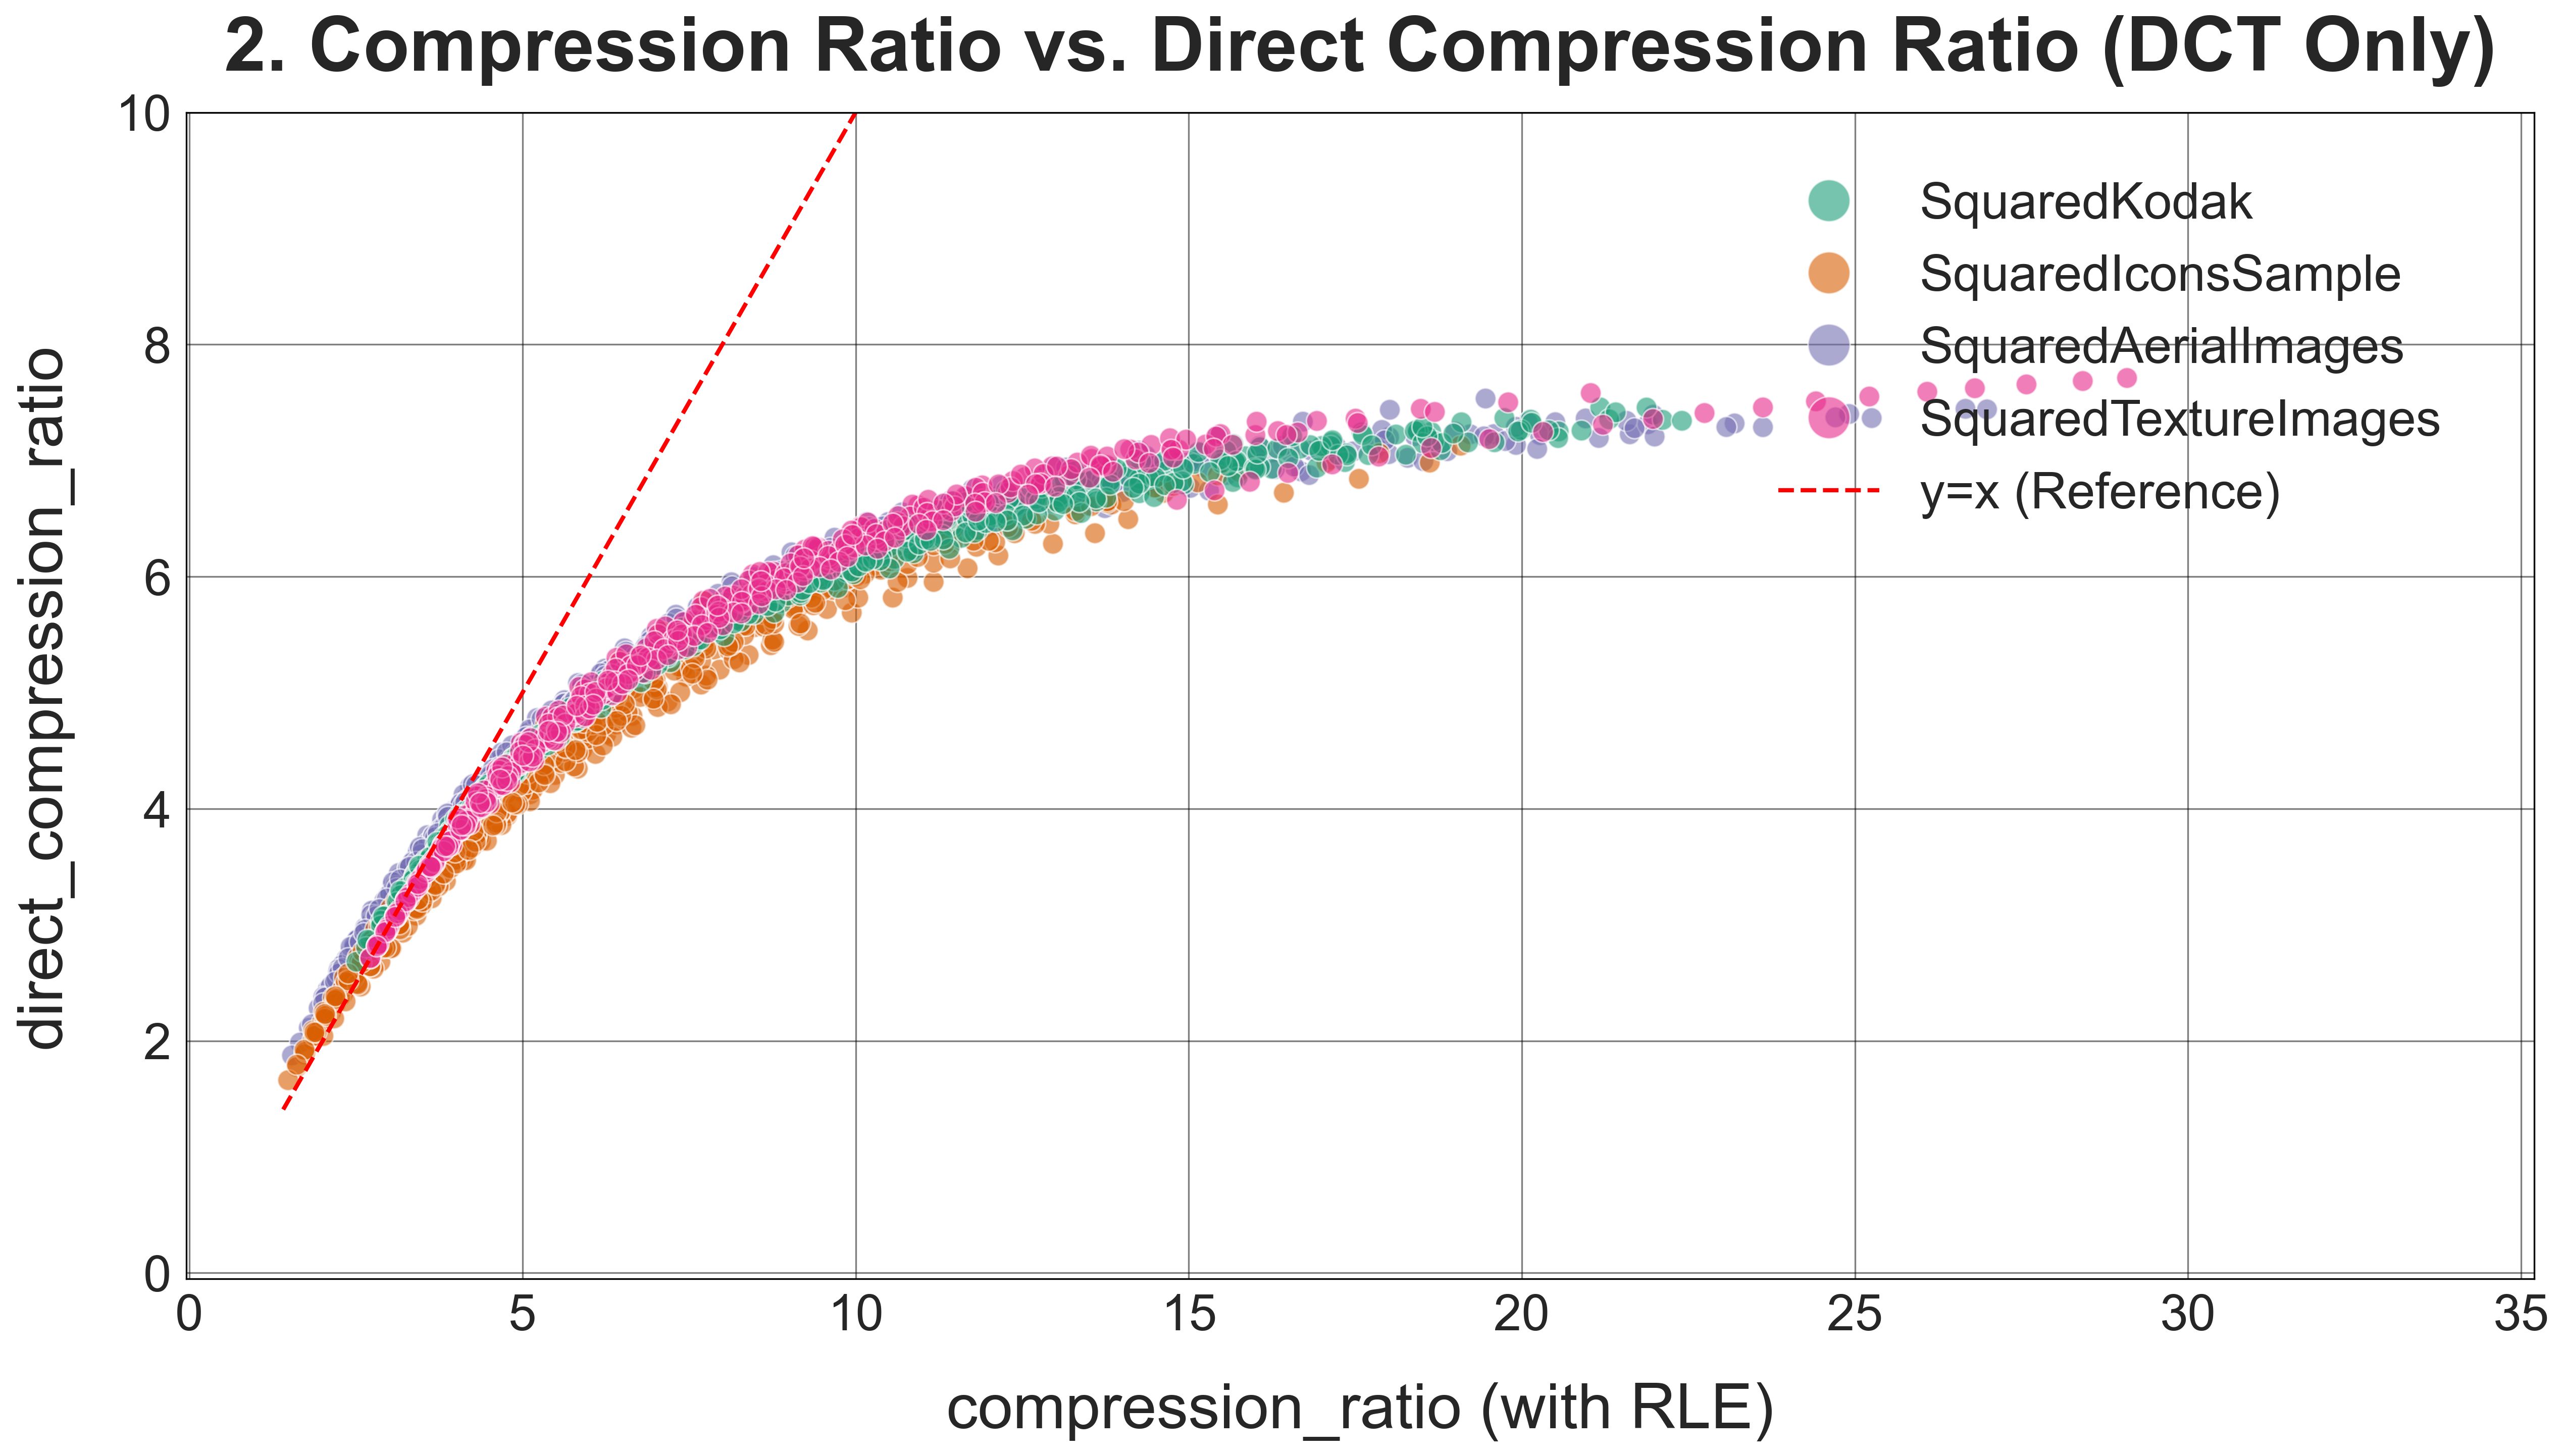
\includegraphics[width=1\linewidth]{results/plots/plot_6_cr_vs_direct_cr_DCT.png}
    \caption{Different levels of quantization on sample image with compression ratio.}
    \label{fig:dctcrvsdcr}
\end{figure}

This provides an excellent example of how compression algorithms can work together to achieve maximum compression for input data. Since the DCT is part of the well established JPEG pipeline, there are lots of extra tools to push the compression to the limit. Likely given more time, other techniques could be implemented to further improve algorithms like DWT and S+P as well.



We claimed in \ref{methodsec:fourier} that DCT is superior to DFT for image compression. To see this clearly, Fig. \ref{fig:dctvsdft} shows how DCT achieves much higher compression ratios at equivalent PSNR values across all datasets. For example, at a PSNR of 30 dB, the DFT achieves CR$\approx5$ across all datasets, while DCT has CR$\approx10$, even closer to 15 for Aerial Images. 

\begin{figure}
    \centering
    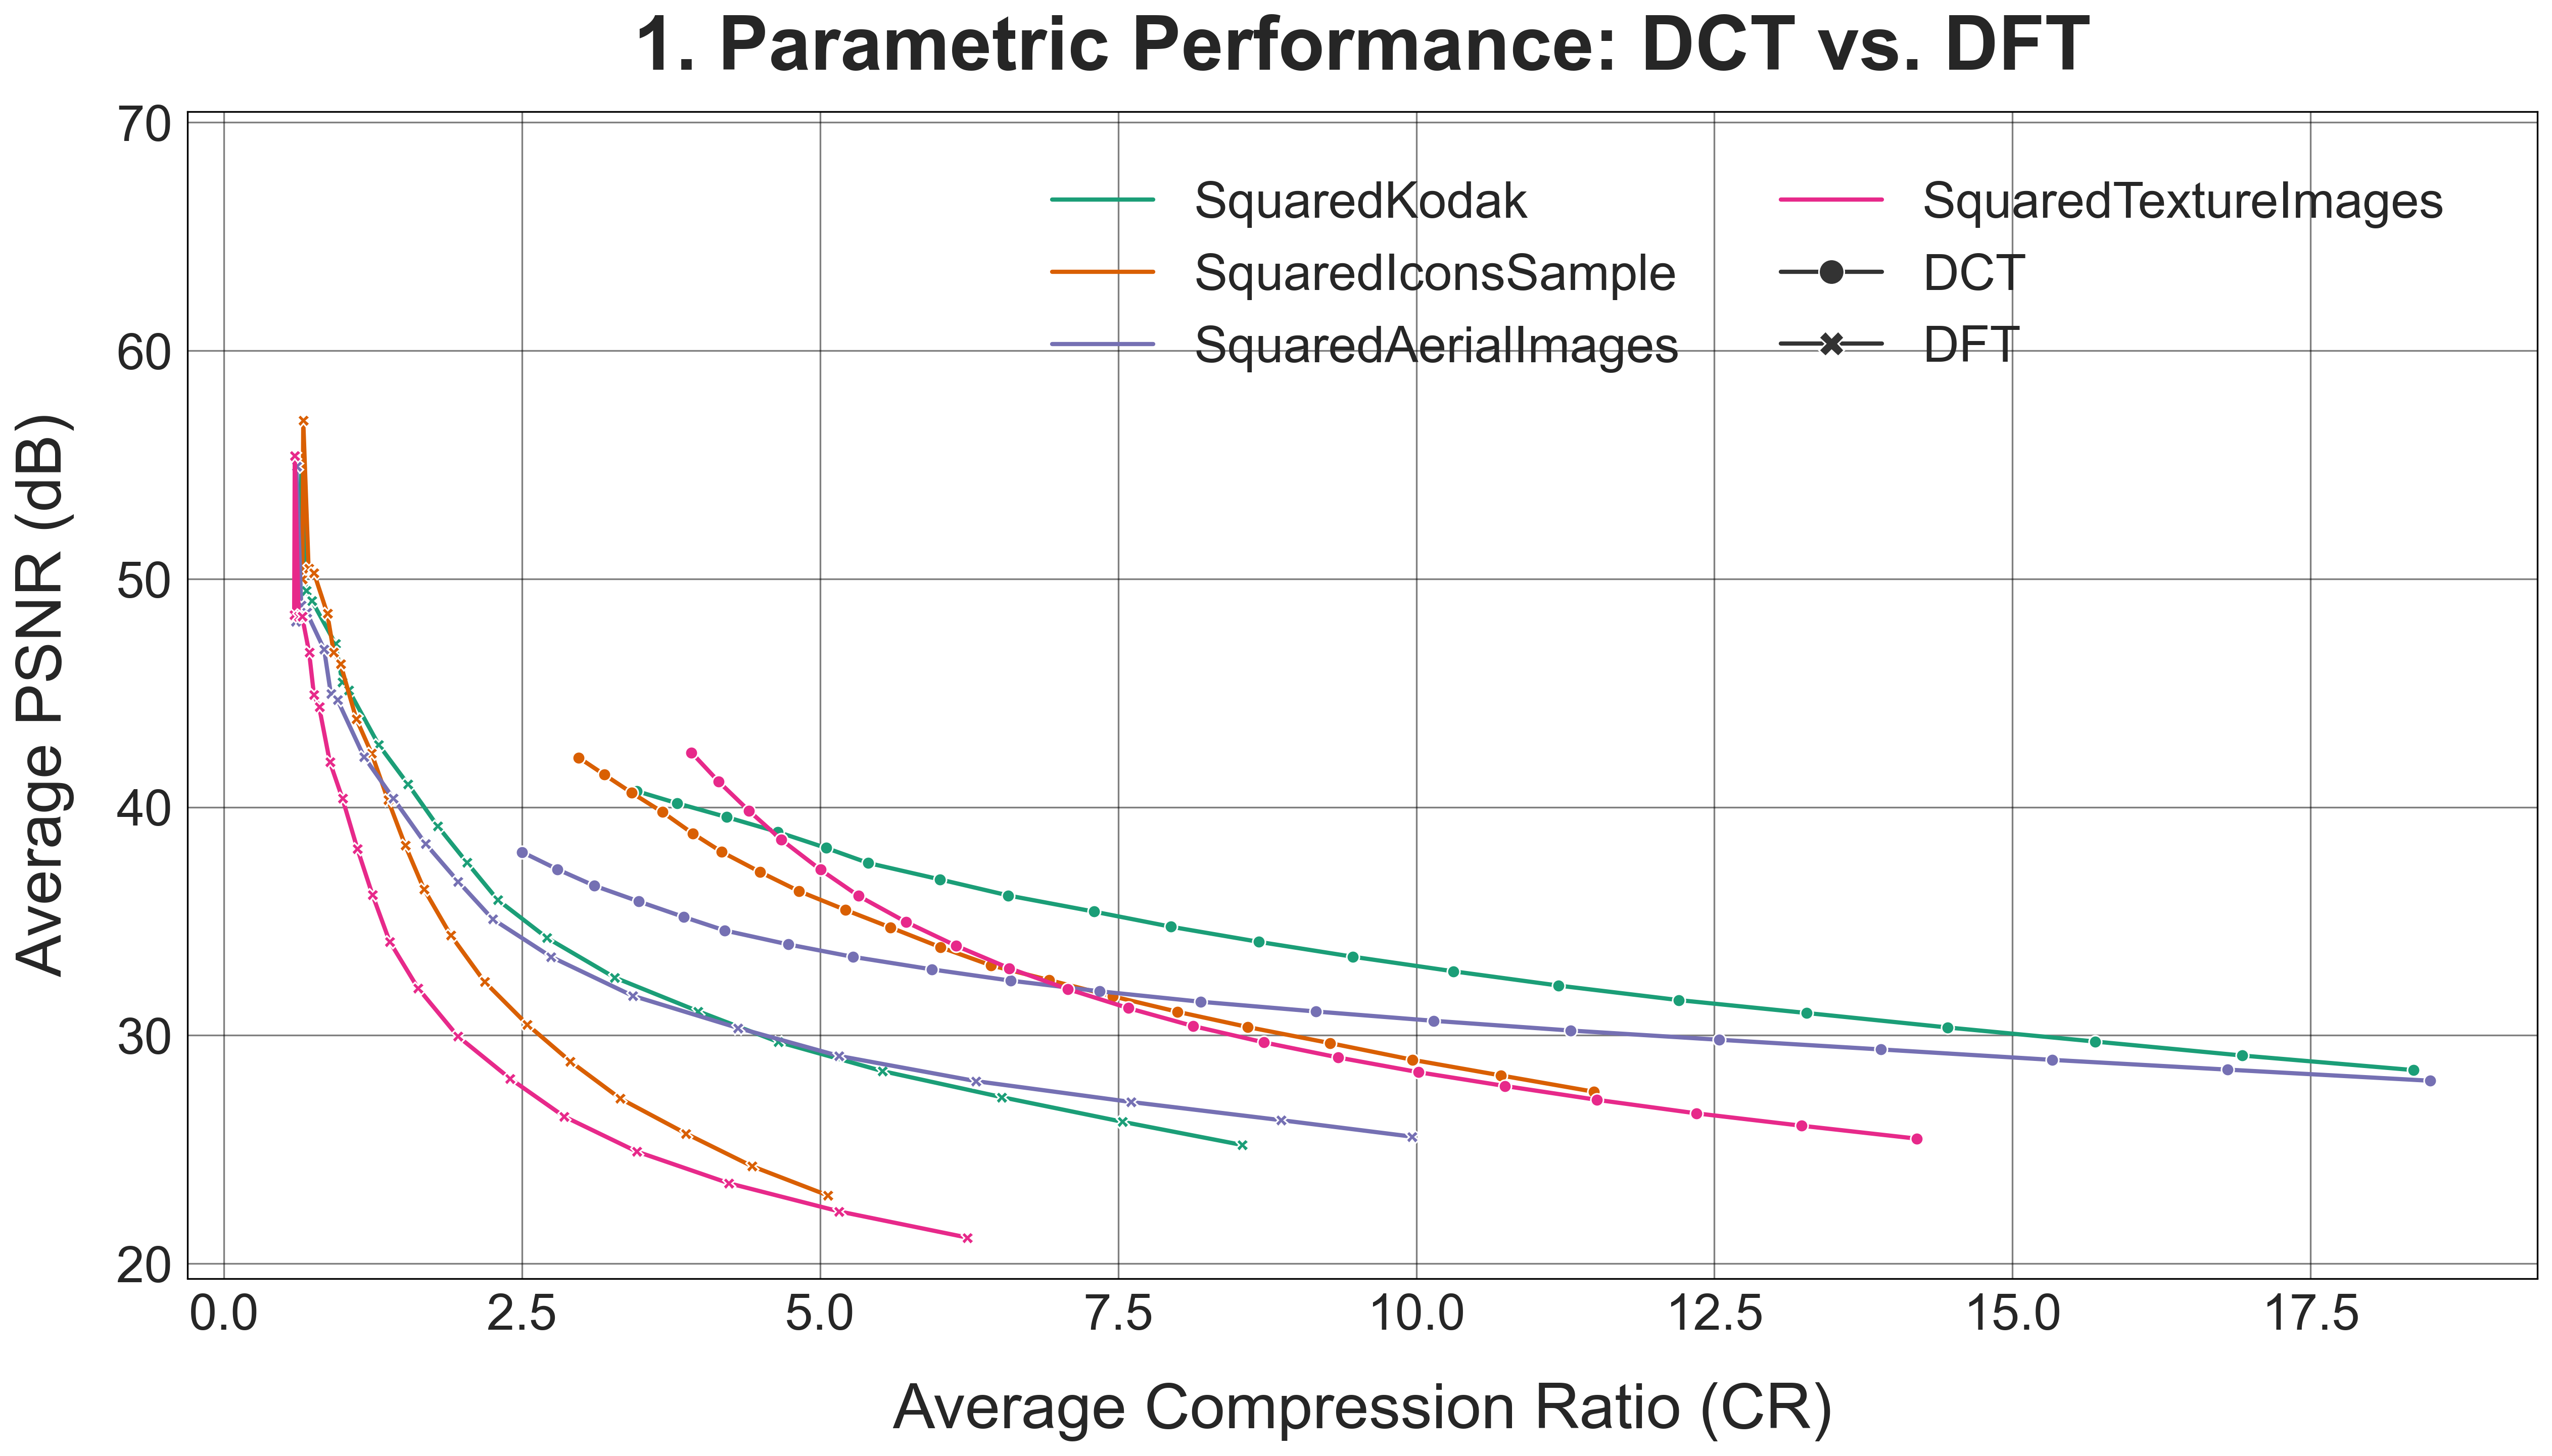
\includegraphics[width=1\linewidth]{results/plots/plot_5_parametric_DCT_vs_DFT.png}
    \caption{Different levels of quantization on sample image with compression ratio.}
    \label{fig:dctvsdft}
\end{figure}

Notably, in \ref{resultssec:col} it appears that the DCT outperforms all transform algorithms, not just the DFT. This comparison is slightly unfair since an additional step RLE was added to the entropy coding for DCT as described in \ref{methodsec:entropy}. Fig. \ref{fig:dctcrvsdcr} shows how the compression ratios change without RLE present for a more fair comparison.

\begin{figure}
    \centering
    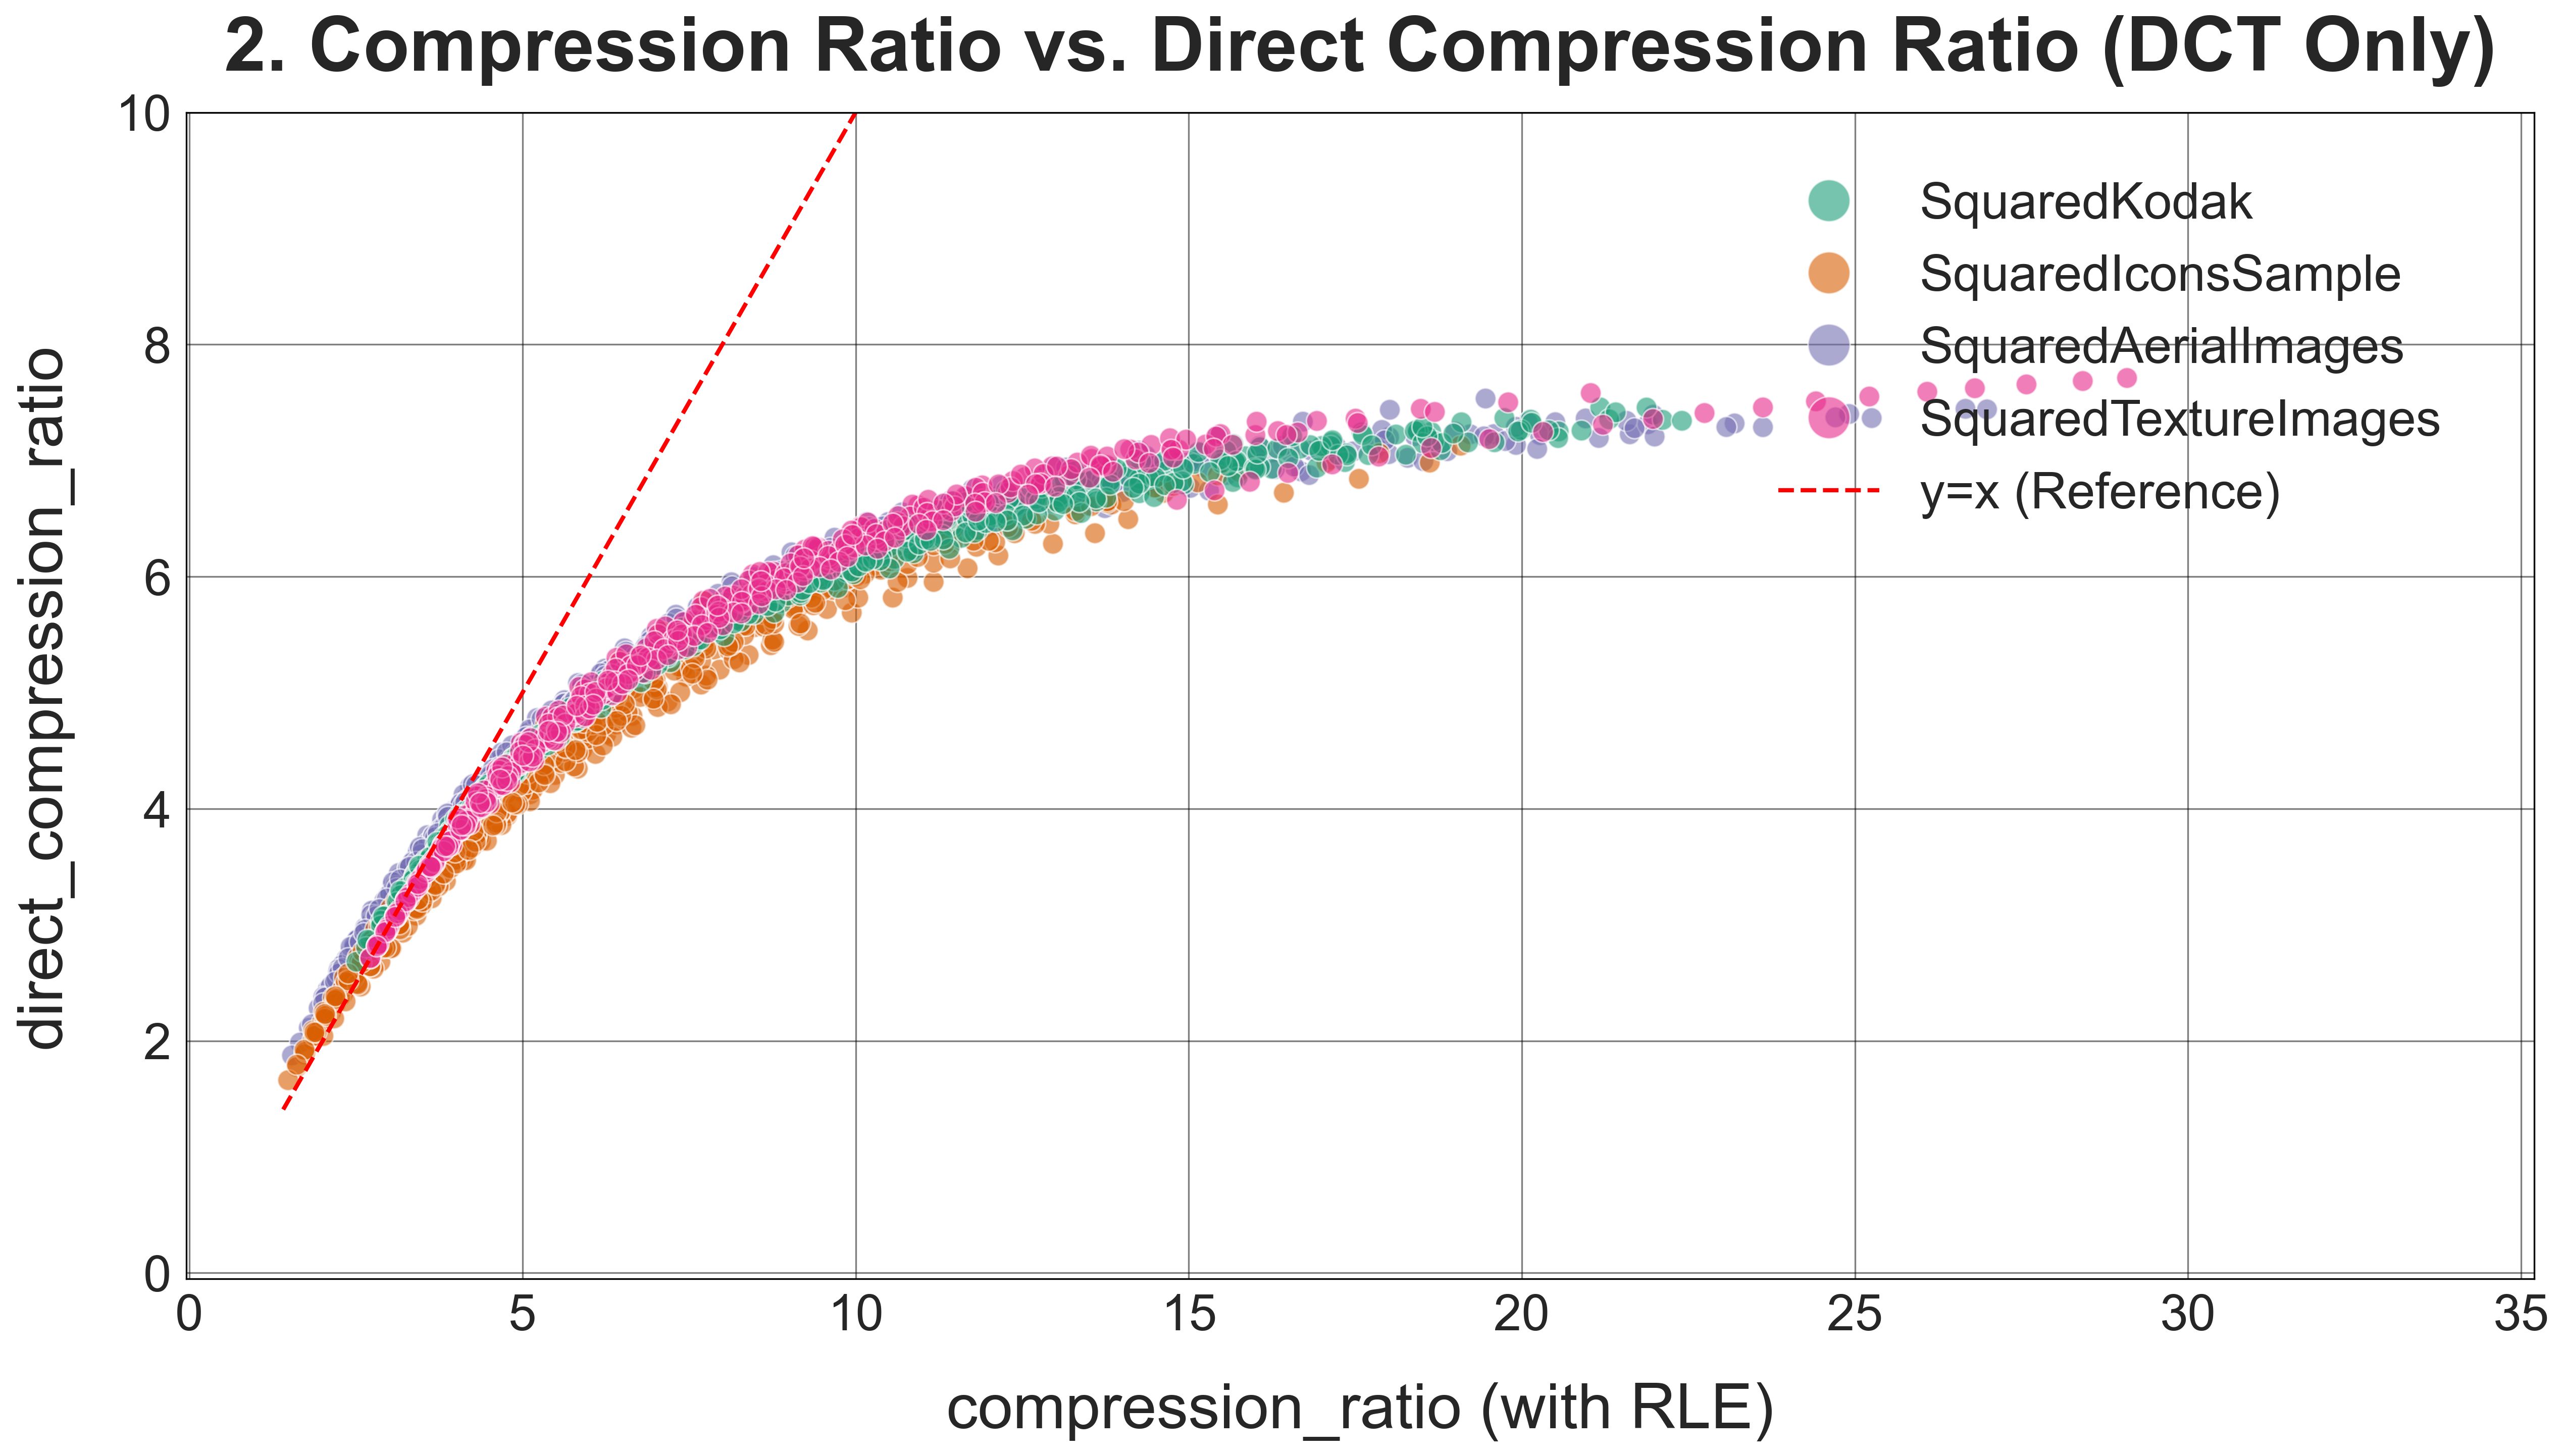
\includegraphics[width=1\linewidth]{results/plots/plot_6_cr_vs_direct_cr_DCT.png}
    \caption{Different levels of quantization on sample image with compression ratio.}
    \label{fig:dctcrvsdcr}
\end{figure}

This provides an excellent example of how compression algorithms can work together to achieve maximum compression for input data. Since the DCT is part of the well established JPEG pipeline, there are lots of extra tools to push the compression to the limit. Likely given more time, other techniques could be implemented to further improve algorithms like DWT and S+P as well.



We claimed in \ref{methodsec:fourier} that DCT is superior to DFT for image compression. To see this clearly, Fig. \ref{fig:dctvsdft} shows how DCT achieves much higher compression ratios at equivalent PSNR values across all datasets. For example, at a PSNR of 30 dB, the DFT achieves CR$\approx5$ across all datasets, while DCT has CR$\approx10$, even closer to 15 for Aerial Images. 

\begin{figure}
    \centering
    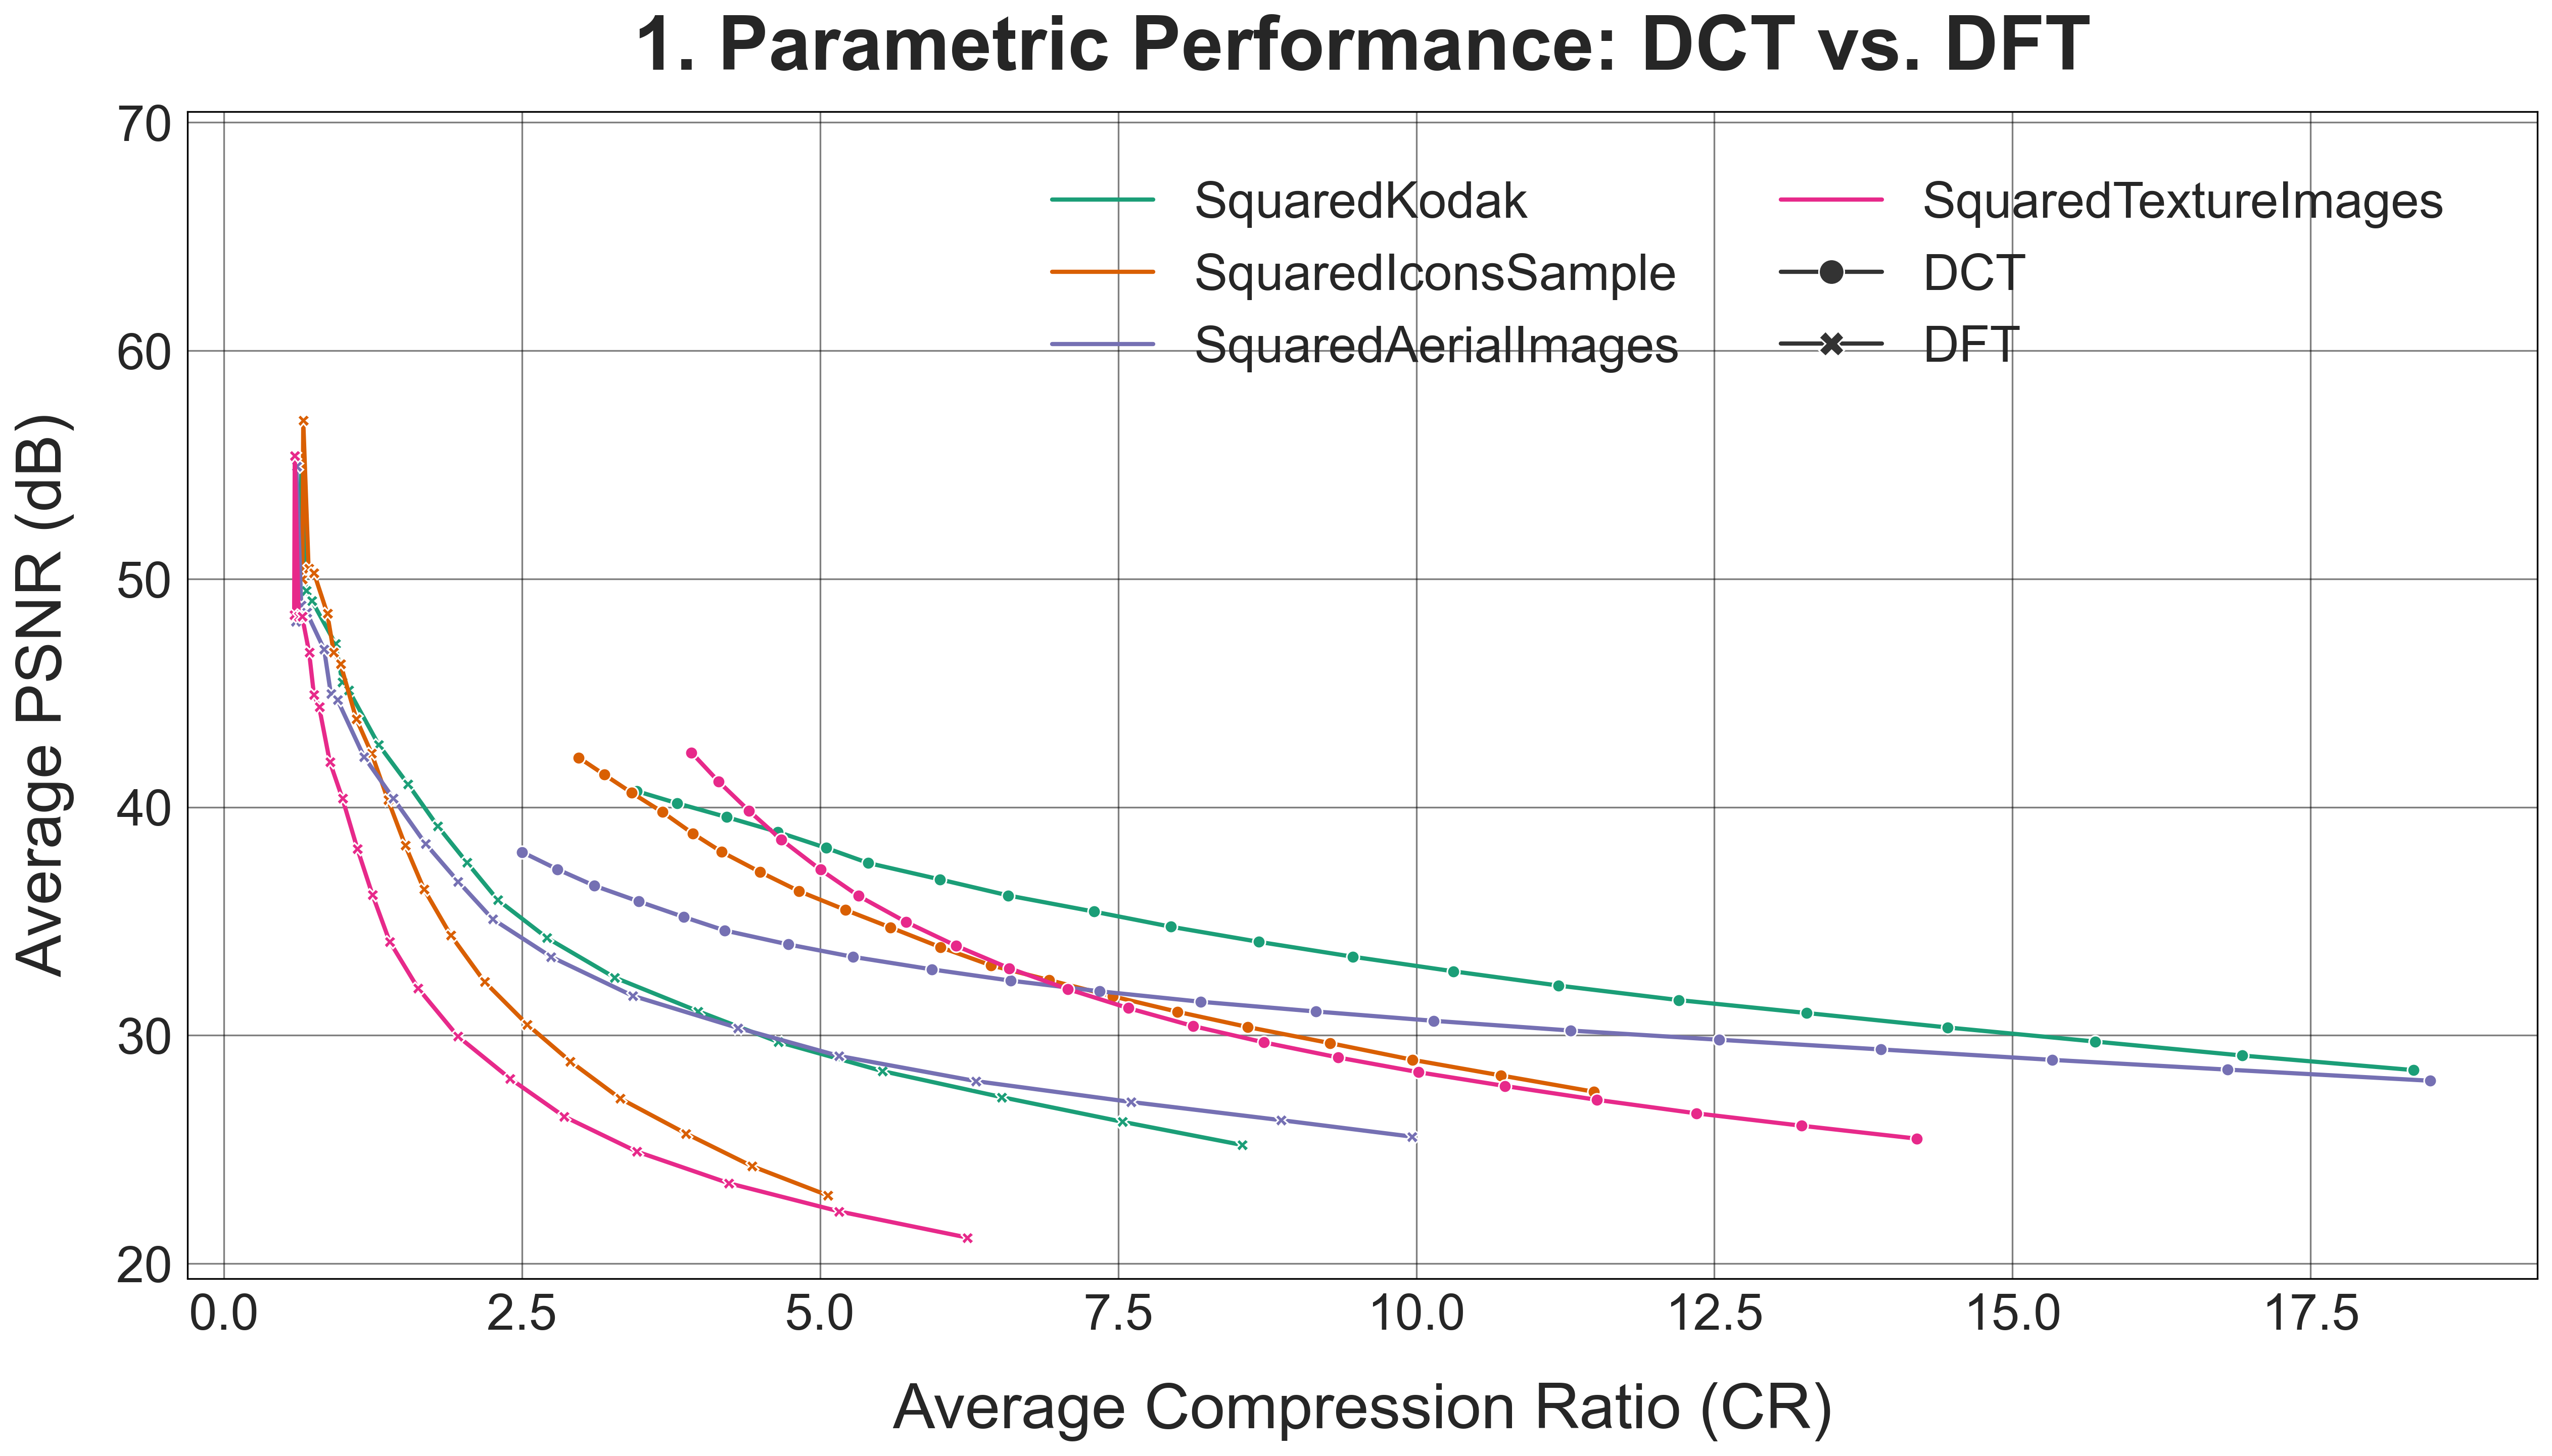
\includegraphics[width=1\linewidth]{results/plots/plot_5_parametric_DCT_vs_DFT.png}
    \caption{Different levels of quantization on sample image with compression ratio.}
    \label{fig:dctvsdft}
\end{figure}

Notably, in \ref{resultssec:col} it appears that the DCT outperforms all transform algorithms, not just the DFT. This comparison is slightly unfair since an additional step RLE was added to the entropy coding for DCT as described in \ref{methodsec:entropy}. Fig. \ref{fig:dctcrvsdcr} shows how the compression ratios change without RLE present for a more fair comparison.

\begin{figure}
    \centering
    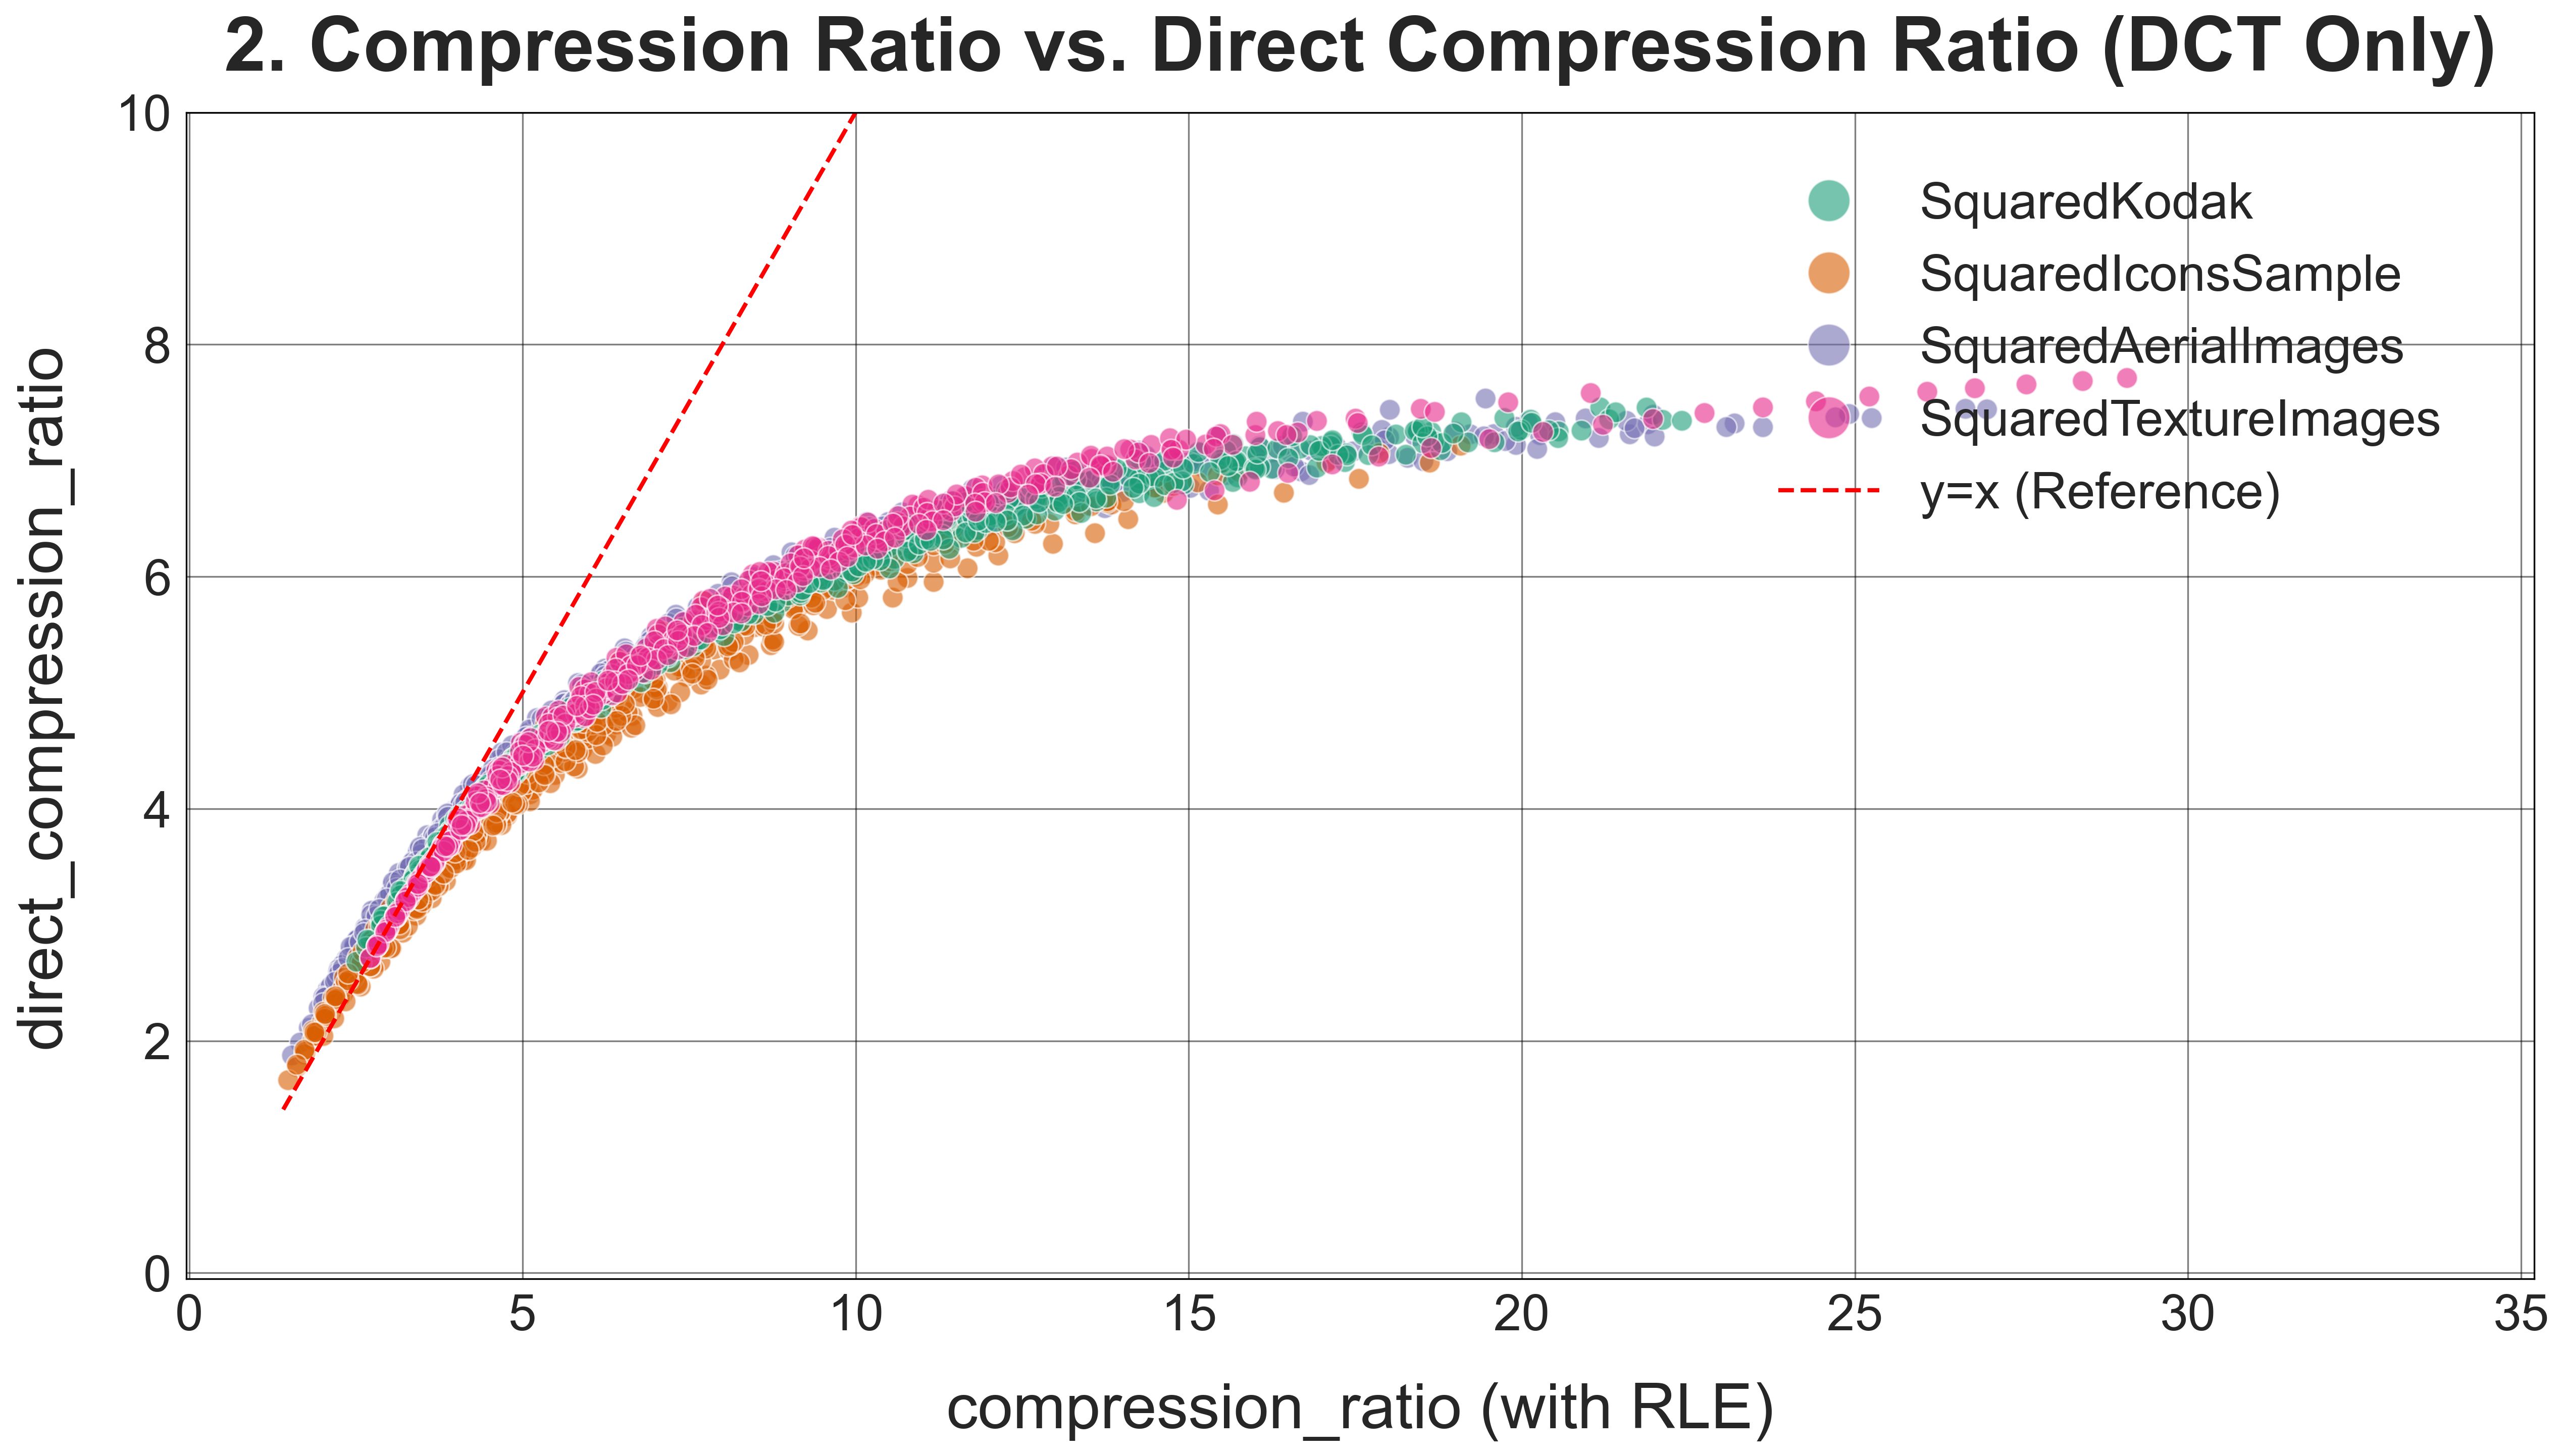
\includegraphics[width=1\linewidth]{results/plots/plot_6_cr_vs_direct_cr_DCT.png}
    \caption{Different levels of quantization on sample image with compression ratio.}
    \label{fig:dctcrvsdcr}
\end{figure}

This provides an excellent example of how compression algorithms can work together to achieve maximum compression for input data. Since the DCT is part of the well established JPEG pipeline, there are lots of extra tools to push the compression to the limit. Likely given more time, other techniques could be implemented to further improve algorithms like DWT and S+P as well.



We claimed in \ref{methodsec:fourier} that DCT is superior to DFT for image compression. To see this clearly, Fig. \ref{fig:dctvsdft} shows how DCT achieves much higher compression ratios at equivalent PSNR values across all datasets. For example, at a PSNR of 30 dB, the DFT achieves CR$\approx5$ across all datasets, while DCT has CR$\approx10$, even closer to 15 for Aerial Images. 

\begin{figure}
    \centering
    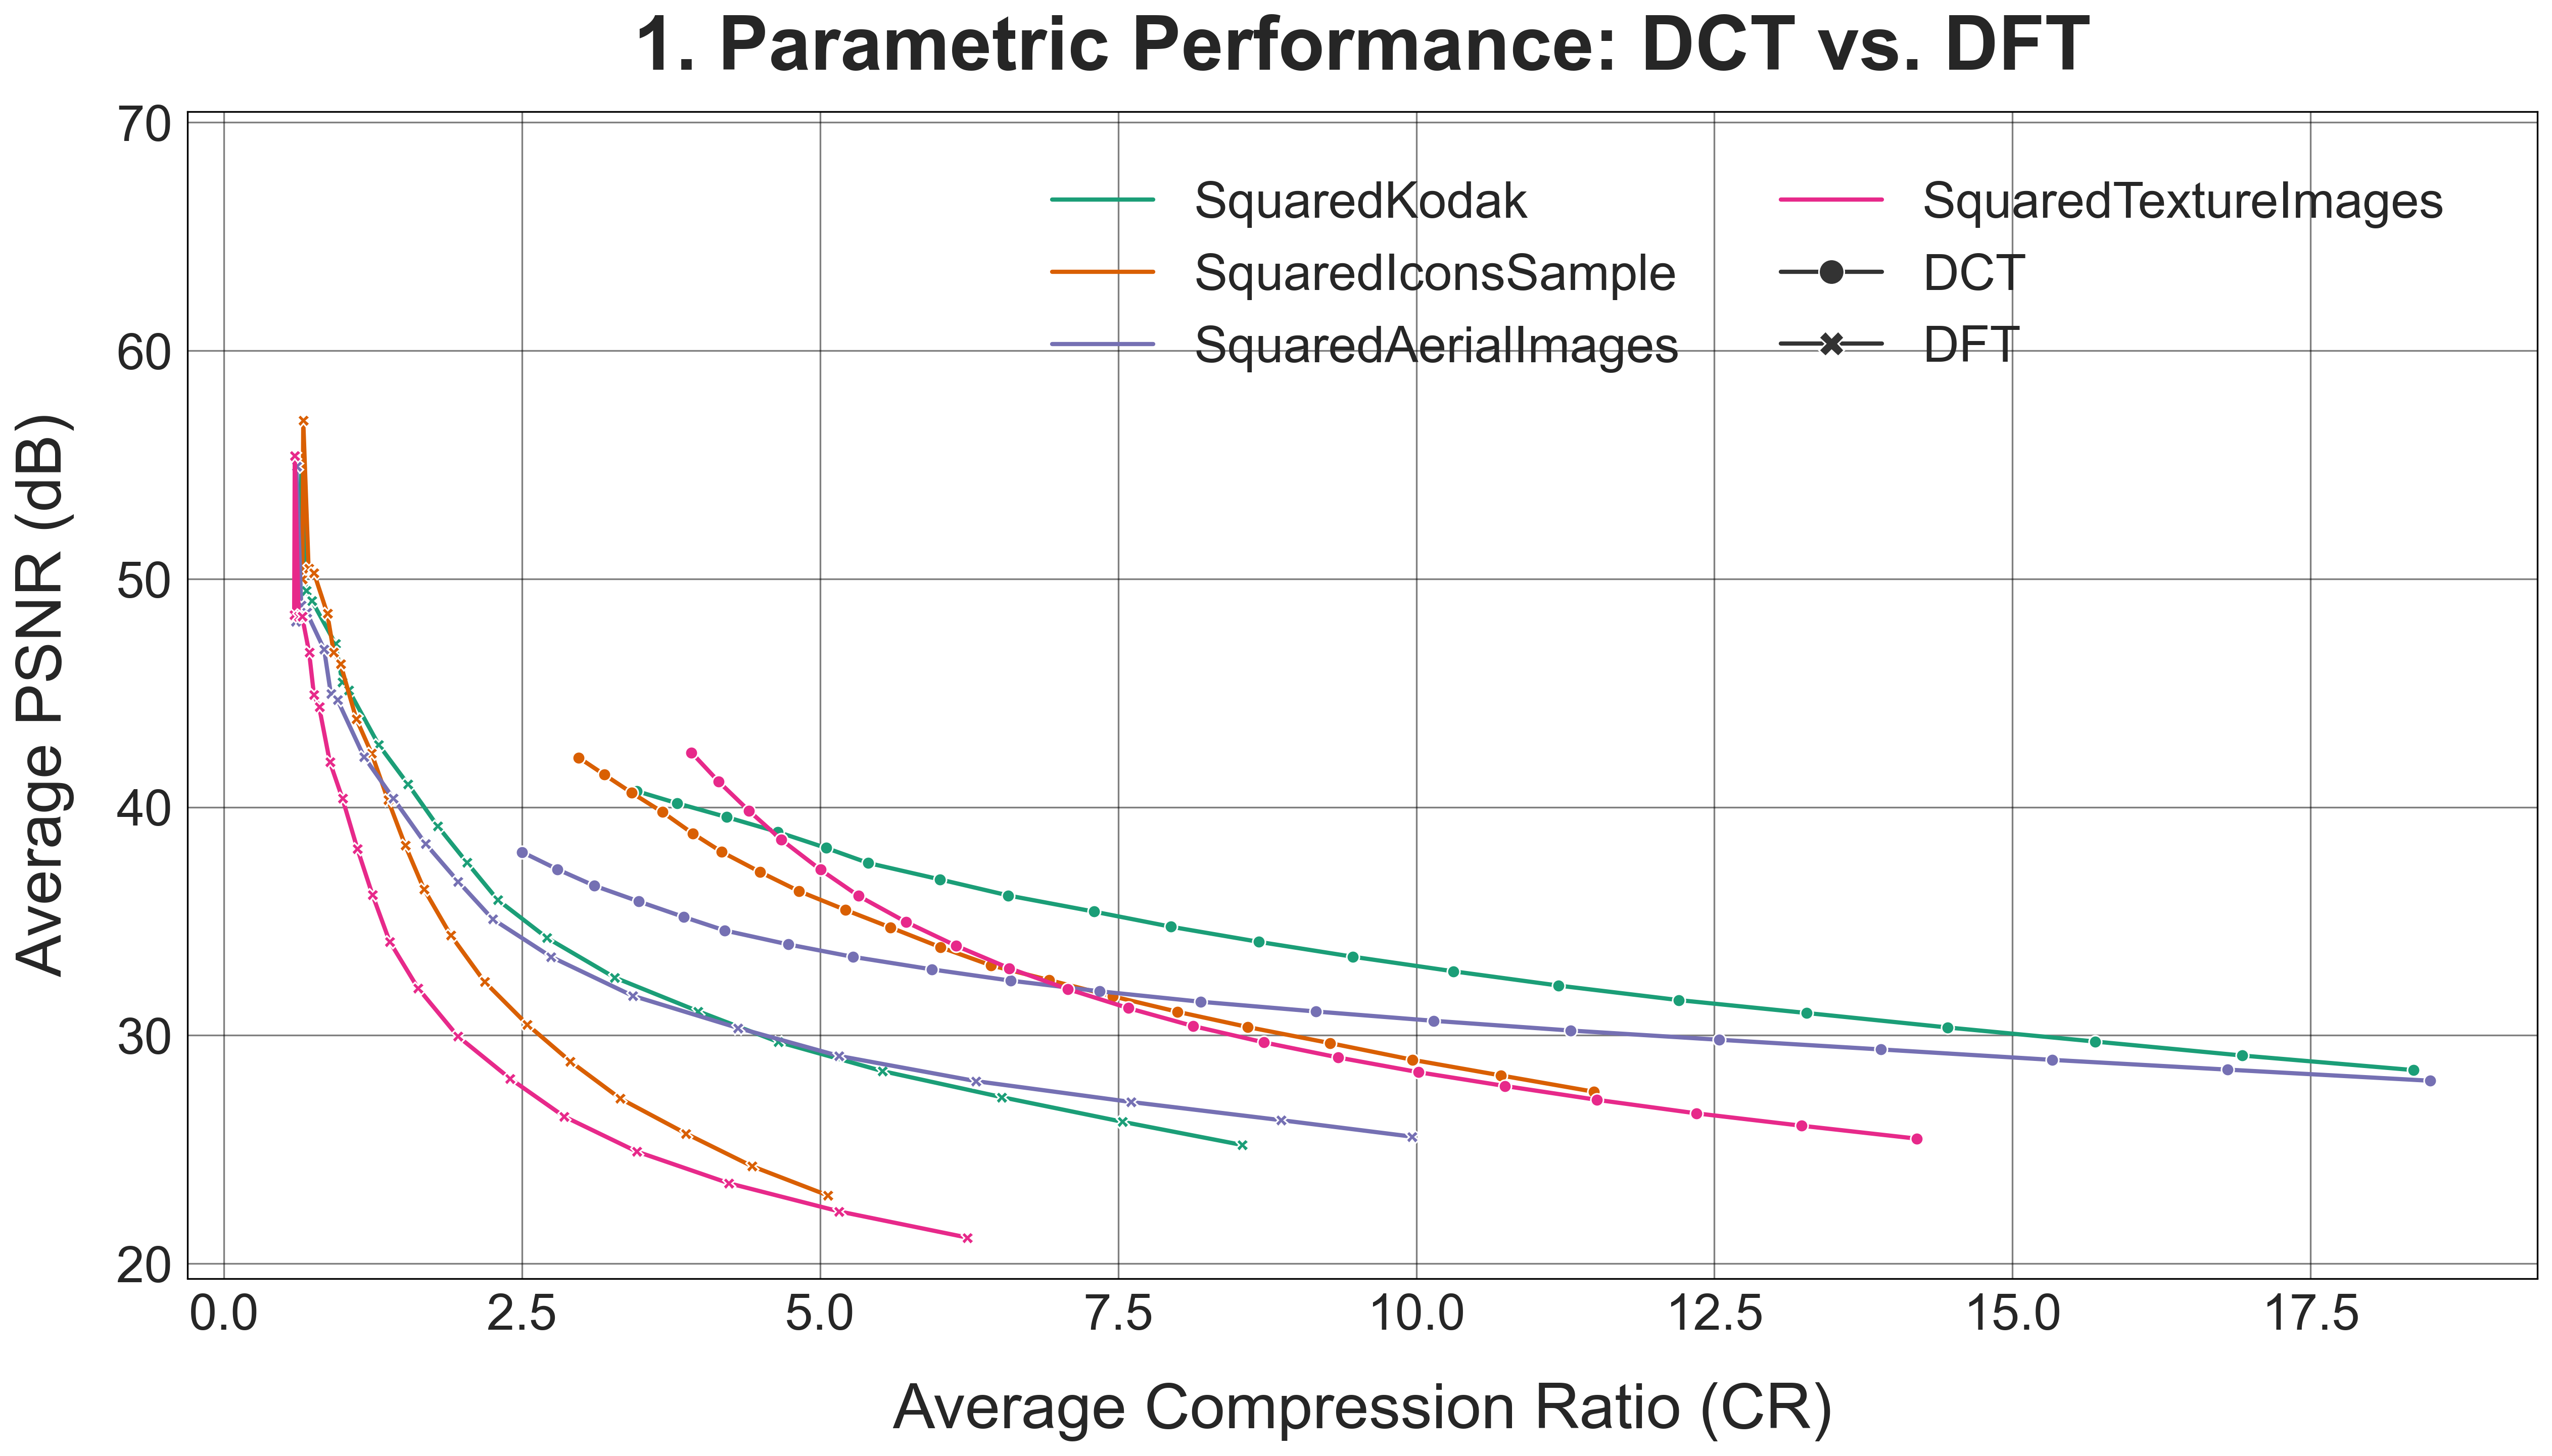
\includegraphics[width=1\linewidth]{results/plots/plot_5_parametric_DCT_vs_DFT.png}
    \caption{Different levels of quantization on sample image with compression ratio.}
    \label{fig:dctvsdft}
\end{figure}

Notably, in \ref{resultssec:col} it appears that the DCT outperforms all transform algorithms, not just the DFT. This comparison is slightly unfair since an additional step RLE was added to the entropy coding for DCT as described in \ref{methodsec:entropy}. Fig. \ref{fig:dctcrvsdcr} shows how the compression ratios change without RLE present for a more fair comparison.

\begin{figure}
    \centering
    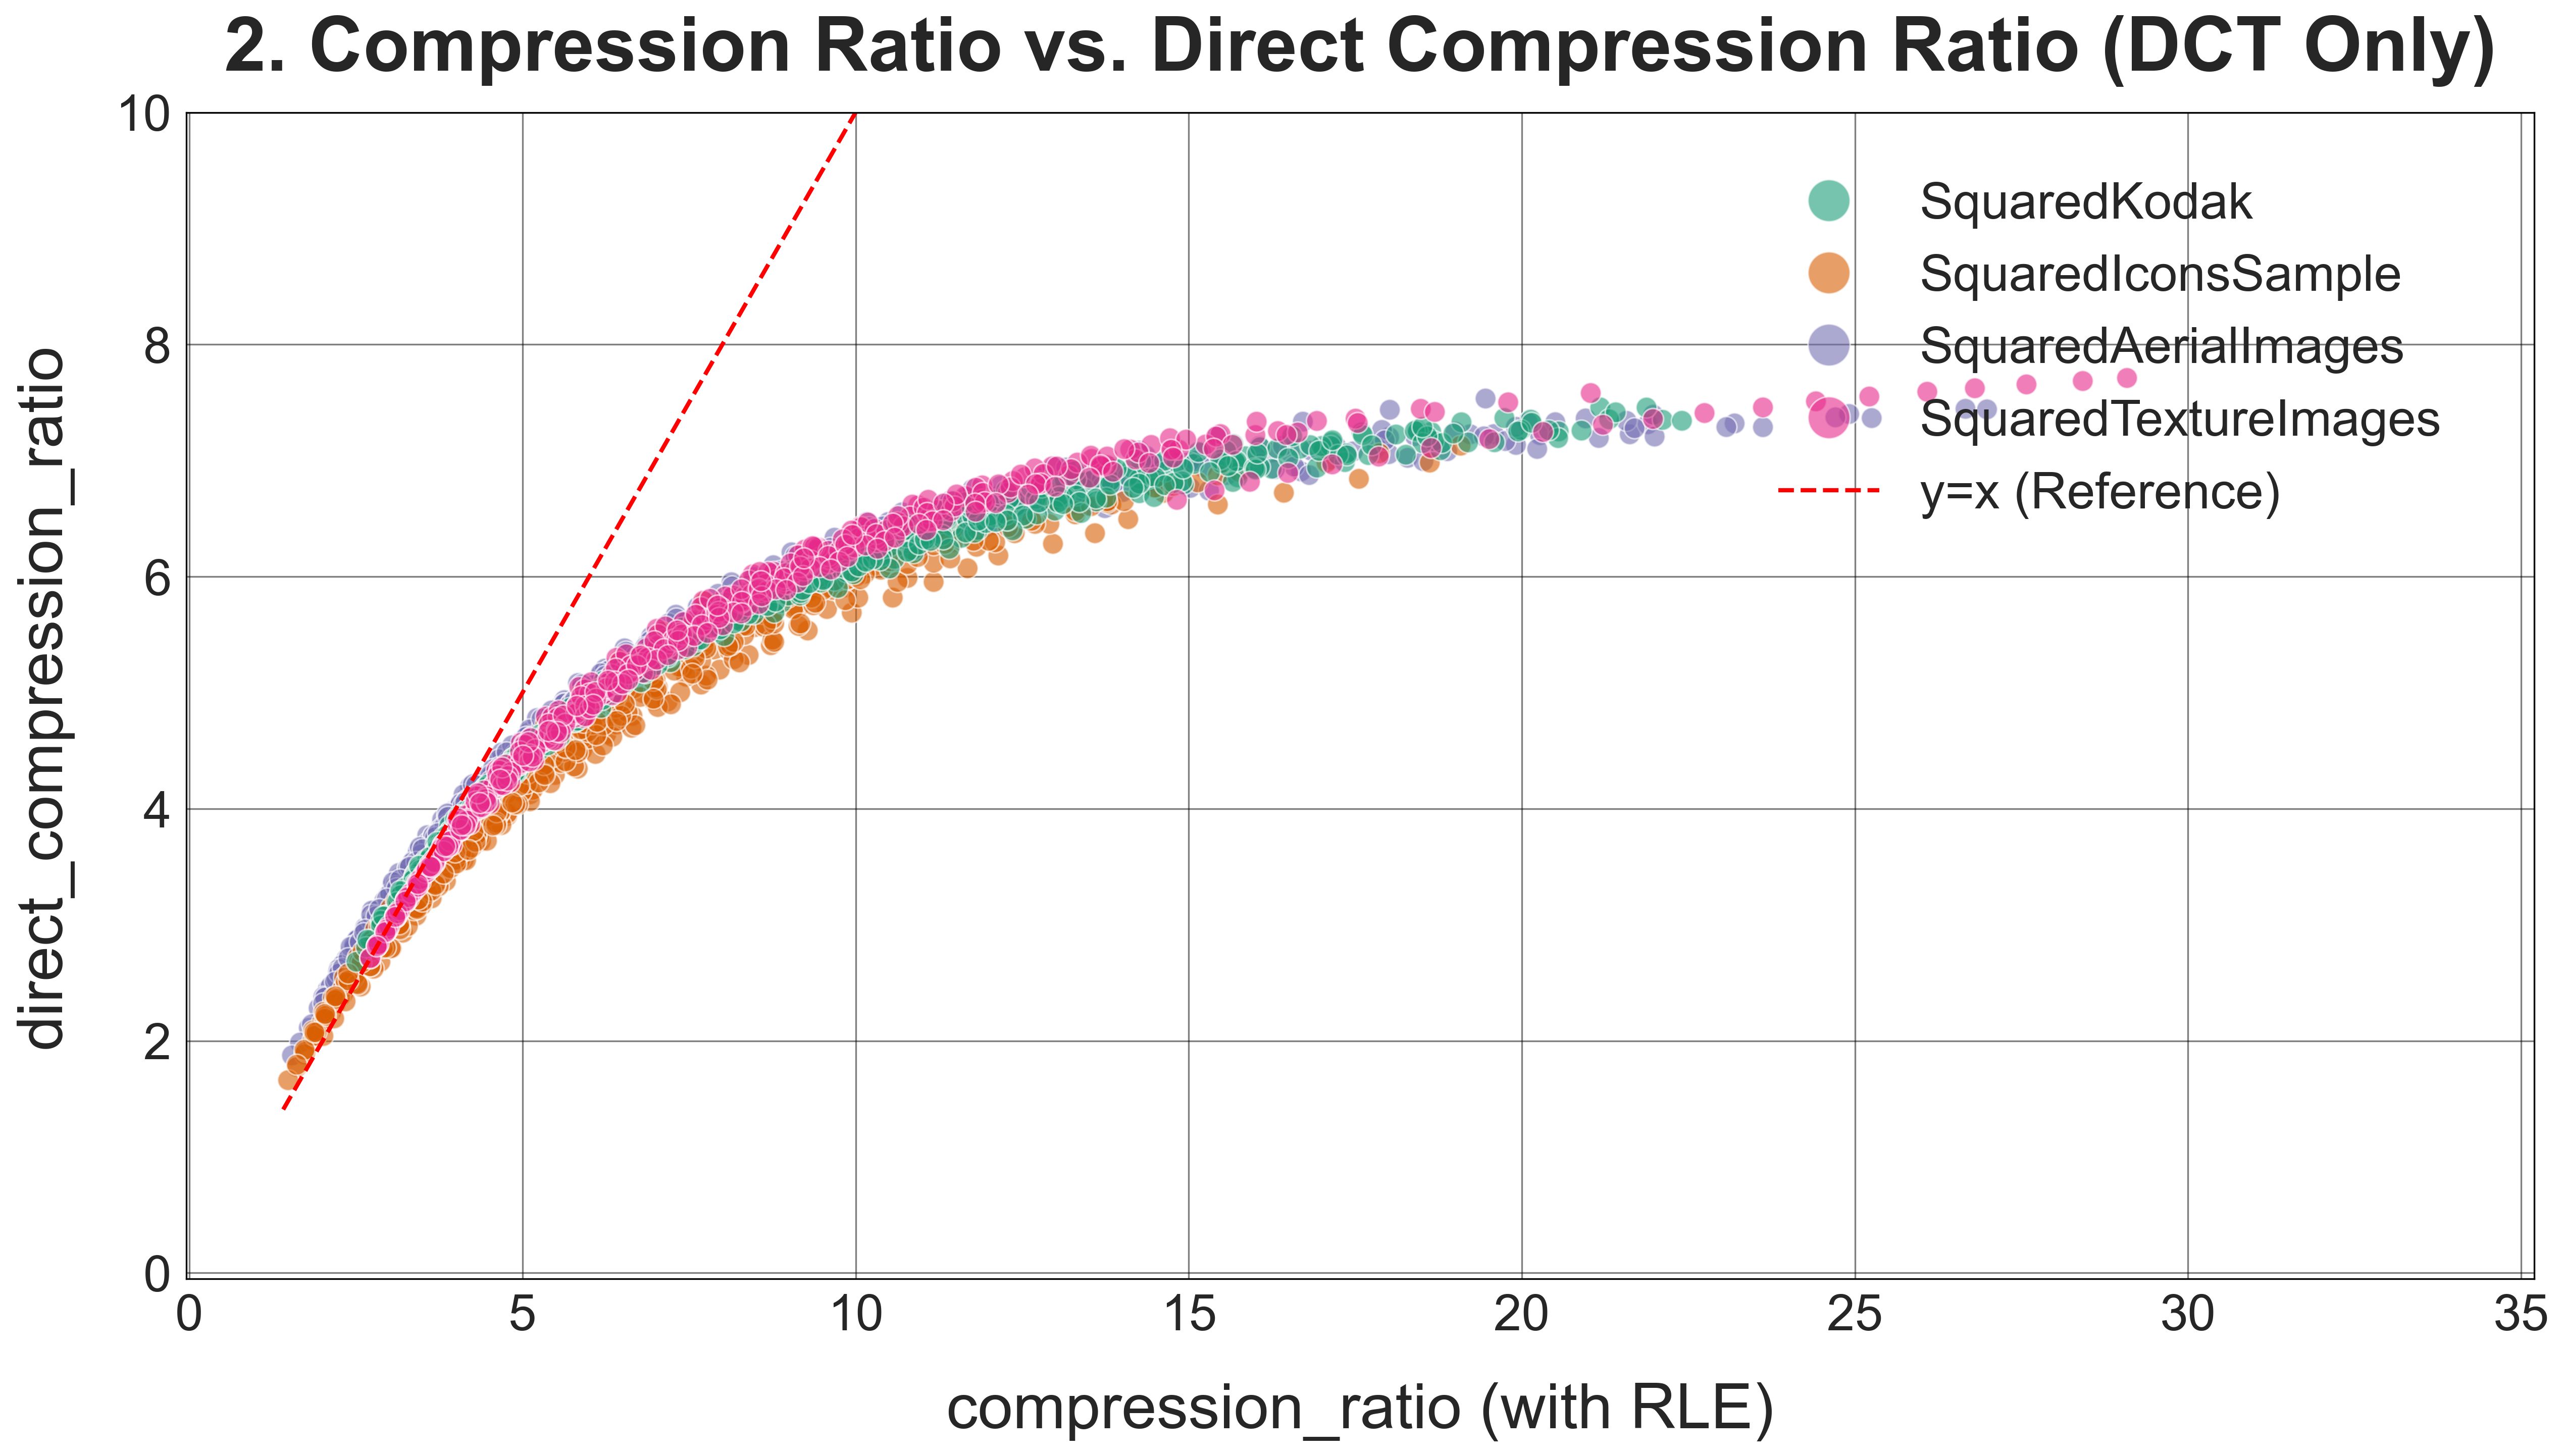
\includegraphics[width=1\linewidth]{results/plots/plot_6_cr_vs_direct_cr_DCT.png}
    \caption{Different levels of quantization on sample image with compression ratio.}
    \label{fig:dctcrvsdcr}
\end{figure}

This provides an excellent example of how compression algorithms can work together to achieve maximum compression for input data. Since the DCT is part of the well established JPEG pipeline, there are lots of extra tools to push the compression to the limit. Likely given more time, other techniques could be implemented to further improve algorithms like DWT and S+P as well.

